% Method: draft notes/draft_method_abstract_review_2026-10-29.md §1 (inbox 20261029-194129), code facts in §0 of that file.
\section{Method}\label{sec:method}
% Facts verified against the code on 2026-10-29: see notes/draft_method_abstract_review_2026-10-29.md §0.

We propose Clean-to-Degraded Two-Pass Distillation (C2D2), a training scheme for multi-sensor segmentation, and apply it to a fusion model built on a frozen vision foundation backbone (Fig.~\ref{fig:arch}). We first describe the model (Sections~\ref{sec:m_backbone}--\ref{sec:m_heads}) and then C2D2 (Section~\ref{sec:m_c2d2}).

% Figure block kept from the previous 4_method.tex (caption to be updated with the router and C2D2 naming).
\begin{figure*}[t]
\centering
% Source: figures/src/fig_arch_standalone.tex + latex/figures/fig_arch.tex (TikZ), built by build.sh.
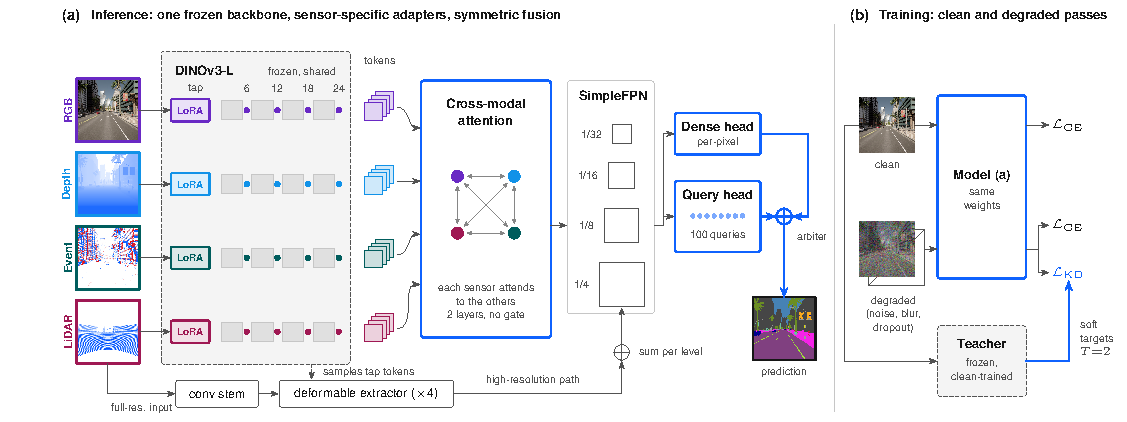
\includegraphics[width=\textwidth]{figures/fig_arch.pdf}
\caption{Overview of \ours{} trained with C2D2. (a) Each sensor passes through the same frozen DINOv3-L with its own LoRA adapter; tokens from four depths are fused by cross-modal attention, decoded by a SimpleFPN augmented with a high-resolution path, and classified by a dense head and a query head combined by an arbiter. (b) C2D2: every batch is used twice, a clean pass and a synthetically degraded pass, the latter also distilled from a frozen teacher trained on clean inputs. Blue outlines mark trained components; dashed boxes are frozen. \todo{add the sensor router to the drawing or caption (FU-01); redraw per notes/figure\_guide.md}}
\label{fig:arch}
\end{figure*}

\subsection{Frozen Backbone with Sensor-Specific Adapters}\label{sec:m_backbone}
Let $x_s$ denote the input of sensor $s\in\{1,\dots,S\}$, converted to a three-channel image (Section~\ref{sec:exp}). Every $x_s$ is processed by the same DINOv3 ViT-L/16 backbone~\cite{dinov3_2025}, whose weights are frozen. Each sensor has its own low-rank adapters (LoRA)~\cite{lora2022} of rank 8 on the query and value projections of every attention block, so that each sensor can adapt the shared features to its own statistics. We take the token maps after blocks 6, 12, 18, and 24 and project each with a sensor-specific $1\times1$ layer, which gives a stride-16 token map $T_s$ per sensor.

\subsection{Cross-Modal Fusion}\label{sec:m_fusion}
Each sensor attends to all other sensors. In each of two layers, the tokens of sensor $s$ form the queries of a multi-head attention whose keys and values are the tokens of the other sensors,
\begin{equation}
\hat{T}_s \leftarrow \hat{T}_s + \mathrm{MHA}\big(\hat{T}_s,\ [\hat{T}_{s'}]_{s'\neq s}\big), \qquad \hat{T}_s^{(0)} = T_s,
\end{equation}
followed by a feed-forward layer. The attention weights are shared across sensors, so every sensor is treated by the same operation. The fused map is the average of the attended maps plus a sensor-specific residual,
\begin{equation}
F = \frac{1}{S}\sum_{s}\hat{T}_s + \sum_{s}\tanh(\gamma_s)\, m_s(T_s),
\end{equation}
where $m_s$ is a small MLP and $\gamma_s$ is a learned scalar per sensor, initialized at 0.1.

\subsection{Sensor Router}\label{sec:m_router}
Each sensor also has an auxiliary head that predicts class logits $A_s$ from $T_s$ and is trained with cross-entropy. A per-class router mixes these predictions pixel by pixel. Its weights are
\begin{equation}
w_{s,k}(p) = \operatorname{softmax}_{s}\big( h_{s,k}(T_s)(p) + \lambda\, r_s(p) \big),
\end{equation}
where $r_s = 1 - H(\sigma(A_s))/\log K$ is the normalized confidence of the auxiliary prediction of sensor $s$ (with gradients stopped), $K$ is the number of classes, and $h_s$ is a small network whose last layer is initialized at zero, so that routing starts from confidence alone. The routed logits $R_k=\sum_s w_{s,k} A_{s,k}$ are added to the final prediction with a learned scale $\alpha$ initialized at zero (Section~\ref{sec:m_heads}). The router is supervised with cross-entropy on $R$ and with a regularizer that favours decisive per-pixel weights. \todo{role of the router after FU-01 (DRN-261029-06/07/08)}

\subsection{Decoder with a High-Resolution Path}\label{sec:m_decoder}
A SimpleFPN~\cite{vitadapter2023} turns $F$ into a feature pyramid at strides 4, 8, 16, and 32. Because every level is interpolated from stride-16 tokens, structures thinner than a token are poorly represented. We therefore add a high-resolution path that follows the adapter of the official DINOv3 segmentation code~\cite{dinov3_2025,vitadapter2023}. A convolutional stem shared across sensors, followed by sensor-specific $1\times1$ projections, extracts multi-scale features from the raw inputs. Deformable-attention extractors, one for each tapped block and two more after the last, let these convolutional features sample semantic evidence from the tapped token maps. Unlike the original adapter, nothing is injected back into the backbone, which stays untouched. The output of the path is added to the FPN levels.

\subsection{Dense and Query Heads}\label{sec:m_heads}
A dense convolutional head classifies every pixel at stride 4 and gives logits $D$. A Mask2Former-style query head~\cite{mask2former2022} with 100 queries and six decoder layers attends to the token maps of all sensors, tagged with a sensor embedding, and its class and mask predictions are converted into per-pixel class scores $Q$. The final logits are
\begin{equation}
\ell_k(p) = D_k(p) + \operatorname{softplus}(\lambda_k)\, Q_k(p) + \alpha\, R_k(p),
\end{equation}
with a learned per-class weight $\lambda_k$. During training, each step uses the dense head alone, the query head alone, or both, with probabilities 0.25, 0.25, and 0.5, so that neither head can rely on the other; at inference both are used.

\subsection{Clean-to-Degraded Two-Pass Distillation}\label{sec:m_c2d2}
C2D2 uses every training batch $(x, y)$ twice.

\emph{Clean pass.} The model sees the clean inputs $x$ and is trained with the segmentation loss $\mathcal{L}_{\mathrm{clean}}$, which combines online hard-example cross-entropy~\cite{ohem2016} on $\ell$ with the losses of the query head, the auxiliary sensor heads, and the router, and two regularizers listed in Section~\ref{sec:exp}.

\emph{Degraded pass.} The model sees a degraded copy $\tilde{x}$. Each sensor of each sample is corrupted independently with probability 0.5. One fifth of the corrupted sensors are removed entirely by setting their normalized input to zero; the others receive one operator drawn from a sensor-specific set: patch dropout, blur, and gain and gamma changes for all image-like sensors, a colour shift for RGB, holes for depth, dropped beams for LiDAR, and resolution loss for events. The corruption strength is capped at 0.3, 0.6, and 1.0 of its maximum from epochs 0, 10, and 20 onward. Gaussian and salt-and-pepper noise are never used in training, so that the noise evaluation tests corruption that the model has not seen. The degraded pass is supervised by the labels and by a frozen teacher $g$, a model of the same architecture without the high-resolution path that was trained on clean inputs with a longer schedule. The teacher sees the clean input:
\begin{equation}
\mathcal{L}_{\mathrm{deg}} = \mathcal{L}_{\mathrm{ce}}\big(\ell(\tilde{x}), y\big) + \beta\, T^2\, \mathrm{KL}\!\left(\sigma\!\left(\tfrac{g(x)}{T}\right) \Big\|\, \sigma\!\left(\tfrac{\ell(\tilde{x})}{T}\right)\right),
\end{equation}
with $\beta=0.5$ and $T=2$, where $\sigma$ is the softmax over classes and the Kullback--Leibler divergence is averaged over pixels. The total loss is $\mathcal{L}_{\mathrm{clean}} + \mathcal{L}_{\mathrm{deg}}$.

C2D2 needs no condition labels and no degradation labels: the degradation is sampled on the fly, and the teacher only sees clean inputs. It changes training only; the model at inference is the same network run once. \todo{after FU-03 (L7, L5, L6): one paragraph on what each part contributes and how C2D2 differs from distillation with missing modalities~\cite{anyseg2024,rmmss2025}}
